\chapter{Разработка собственного решения с использованием белорусской криптографии}

	\section{Поиск существующих имплементаций}
	
	Первой задачей практической части было нахождение существующих реализаций подробно описанных
	выше протоколов с целью дальнейшей работы над криптографическим аспектом этих реализаций.
	В качестве основного протокола для модификаций был выбран протокол ZigBee. Были поставлены
	следующие задачи:
	
	\begin{itemize}
		\item поиск имплементации протокола ZigBee, позволяющей вносить модификации; 
		\item поиск устройств (микроконтроллеров), способных работать на этой имплементации;
		\item изменение или полная замена криптографической составляющей в имплементации.
	\end{itemize}

	К сожалению, открытых реализация оказалось немного. Практически не было найдено библиотек,
	реализующих в полной мере последнюю версию протокола. Проблема заключается в том, что сама
	спецификация находится в закрытом доступе. Для получения спецификации необходимо стать
	членом ZigBee Alliance, что осуществляется на платной основе. Аналогично, все имплементации
	протокола ведущими технологическими компания также являются закрытыми. Это связано с
	коммерческой составляющей, поскольку компании получают прибыль, реализуя устройства
	на собственных прошивках.
	
	По совокупности вышеописанных факторов был выбран другой подход, который не привязан
	к определённому протоколу. Суть данного подхода заключается в самостоятельной реализации
	криптографического уровня защиты и применении его поверх установленного соединения между
	управляющим устройством (хабом) и конечным устройством. В качестве конечного устройства
	в данной работе был выбран прототип умной лампочки.
	
	
	\section{Выбор компонентов и технологий для реализации}
	
	Обновлённые практические задачи были сформулированы следующим образом:
	
	\begin{itemize}
		\item выбор микроконтроллера, который будет служить прототипом умного устройства,
		с возможностью его программирования и прошивки;
		\item установка соединения между управляющим и умным устройствами. Для простоты в качестве
		управляющего устройства в данной работе используется компьютер;
		\item разработка кода (прошивки) для умного устройства (контроллера), а также клиентского
		приложения для управляющего устройства;
		\item реализация защищённого обмена сообщениями с использование белорусского криптографического
		стандарта СТБ 34.101.77;
		\item модификация стандарта с изменением значения некоторых его параметров;
		\item оценка стойкости видоизменённого решения.
	\end{itemize}

	В качестве микроконтроллера был выбран ESP8266 (модель NodeMCU V3). Это недорогая модель от
	китайской компании Espressif Systems. Её большим преимуществом является встроенный Wi-Fi модуль. 
	Помимо поддерживаемых протоколов Wi-Fi 802.11 b/g/n и режимов работы как в качестве точки доступа,
	так и клиента, микроконтроллер отличается встроенным стеком TCP/IP.
	
	Для программирования данной модели существует широкий выбор языков, платформ и сред, среди
	которых Arduino IDE, Espressif IoT Development Framework (официальный фреймворк от разработчика)
	и многие другие. В данной работе был выбран инструмент PlatformIO \cite{platformio}. Это
	кроссплатформенная интегрированная среда разработки, построенная на основе редактора Microsoft 
	Visual Studio Code, а также встроенный отладчик, статический анализатор кода и система сборки.
	Платформа поддерживает большое количество микроконтроллеров, среди которых в том числе есть
	ESP8266 NodeMCU. На сайте также представлен широкий выбор библиотек и примеров с кодом.
	Языком разработки на платформе является C++.
	
	При выборе инструментов и технологий для разработки также рассматривались варианты использования
	более высокоуровневых языков программировая, таких как Java \cite{microej} или .NET \cite{nanoFramework}.
	Однако наличие примеров, библиотек и большого сообщества разработчиков стало определяющим
	фактором при выборе PlatformIO. При этом для клиентского веб-приложения на управляющем устройстве
	(компьютере) был выбран язык программирования Java.
	
	
	\section{Работа с микроконтроллером ESP8266}
	
	\begin{figure}[h]
		\centering
		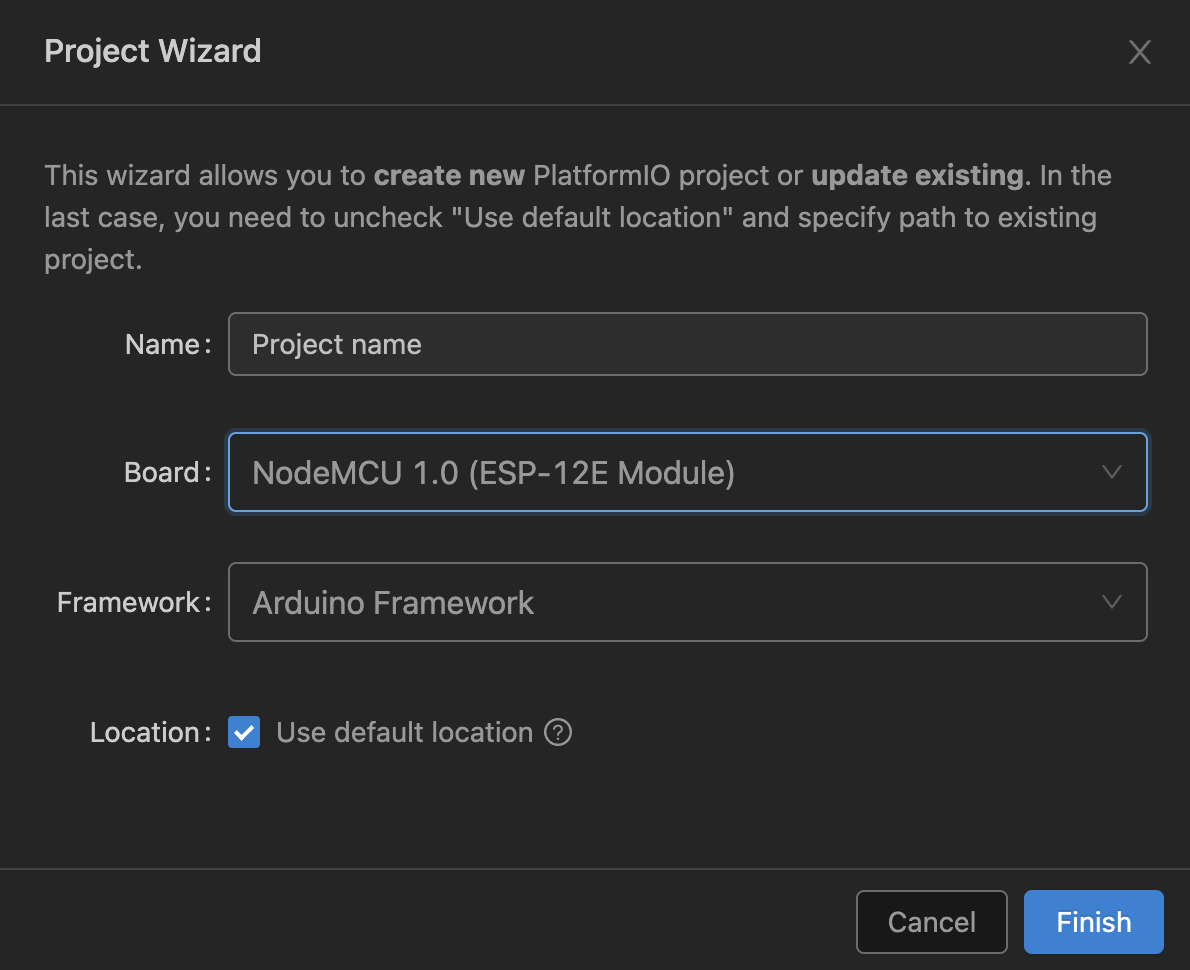
\includegraphics[scale=0.6]{resources/platformio-new-project}
		\caption{Меню создания нового проекта в PlatformIO}
		\label{fig4.1}
	\end{figure}
	
	Первым шагом при программировании микроконтроллера стало создание проекта при помощи PlatformIO.
	На этапе создания нового проекта появляется возможность выбора контроллера. Основными составляющими
	в проекте являются конфигурационный файл platformio.ini, в котором указывается модель контроллера,
	а также подключаемые к проекту библиотеки, и директива src, в которой должен содержаться код проекта.
	
	При первоначально настройке в папке src содержится единственный файл main.cpp. Он включает два
	метода. Метод setup() отвечает за первоначальную конфигурацию контроллера, а метод loop()
	повторяется всё время, пока контроллер подключен к питанию.
	
	Для знакомства с программированием данного типа контроллеров и изучения программных методов
	было реализовано несколько базовых примеров. Первым из них было мигание встроенного на контроллере
	индикатора. Затем были построены простейшие схемы с использованием макетной платы, диода и
	нескольких проводов. Мигание встроенного индикатора было заменено миганием диода. После этого
	был реализован пример управления диода по нажатию кнопки. Наконец, был задействован Wi-Fi модуль
	для управления диодом с компьютера. Данный пример был взят за основу практического прототипа. Более
	подробно работа прототипа и все этапа обмена сообщениями будут рассмотрены позже. Но перед этим
	перейдём к криптографической части данной работы.
	
	\begin{figure}[h]
		\centering
		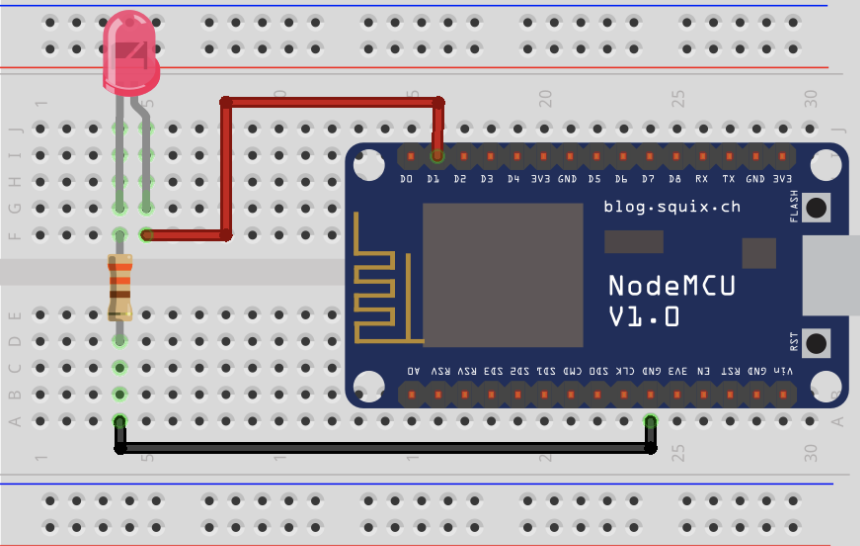
\includegraphics[scale=0.6]{resources/esp8266-control-led}
		\caption{Схема подключения диода к микроконтроллеру}
		\label{fig4.2}
	\end{figure}
	
	
	\section{Реализация и использование криптографического стандарта СТБ 34.101.77}
	
	\subsection{Описание стандарта}
	
	Официальное название стандарта $-$ <<Криптографические алгоритмы на основе sponge-функции>> \cite{standard-77}.
	Разберём для начала, что из себя представляет sponge-функция.
	
	Sponge-функция $-$ это класс алгоритмов с конечным внутренним состоянием. Эти алгоритмы
	предназначены для обеспечения конфиденциальности, целостности и подлинности информации
	при её передачи и обработке. Сама функция задаёт сложное преобразование двоичных слов большой 
	длины. Криптографические алгоритмы подразделяются на две большие группы:
	
	\begin{enumerate}
		\item алгоритмы хэширования, описанные в разделе 7 стандарта;
		\item программируемые алгоритмы, описанные в разделе 8.
	\end{enumerate}

	В практической части данной работы используются только программируемые алгоритмы, в частности
	алгоритмы аутентифицированного шифрования, которые представляют собой последовательности 
	команд криптографического автомата. Более подробно о них речь пойдёт далее.

	Стандарт описывает преобразование двоичных слов длины 1536 бит (192 байта). Преобразование
	задаётся алгоритмом bash-f, который в свою очередь использует алгоритм bash-s. bash-f и bash-s
	являются sponge-функциями, которые определяют программируемые алгоритмы. Стандартные уровни
	стойкости $l = 128, 192, 256$. Дополнительным параметром является ёмкость $d \in \{1, 2\}$.
	В программируемых алгоритмах также используется ключ $K$, длина которого должна быть не меньше 
	уровня стойкости, но также не превосходить 480. Для контроля целостности и подлинности вычисляется
	имитовставка, длина которой равна уровню стойкости $l$.
	
	Управление автомата, лежащего в основе программируемых алгоритмов, осуществляется командами.
	Допустимы следующие команды:
	
	\begin{itemize}
		\item start (инициализация). На этом этапе происходит загрузка ключа;
		\item restart (повторная инициализация);
		\item absorb (загрузка данных);
		\item squeeze (выгрузка данных). С помощью этой команды осуществляется вычисление имитовставки;
		\item encrypt (операция зашифрования);
		\item decrypt (операция расшифрования);
		\item ratchet (необратимое изменение состояния автомата);
		\item commit (подтверждение выполнения других комманд).
	\end{itemize}

	В практической части данной работы были реализованы команды start, absorb, squeeze, encrypt, 
	decrypt, commit. Все перечисленные команды используются в аутентифицированном шифровании,
	которое и применяется для защиты данных, передаваемых между умными устройствами. Алгоритм
	установки защиты заключается в последовательном применении команд start, absorb, encrypt, squeeze,
	а алгоритм снятия защиты выполняет команды start, absorb, decrypt и squeeze соотвественно.
	
	\subsection{Практическая реализация}
	
	Алгоритмы bash-s и bash-f являются низкоуровневыми, поскольку оперируют с битами. Поэтому они 
	были реализованы на языке программирования C. Так как язык прошивки микроконтроллера $-$ C++,
	а язык клиентского приложения $-$ Java, команды для управления автоматом при аутентифицированном 
	шифровании необходимо было реализовать на двух этих языках. Рассмотрим сначала реализацию на Java.
	
	Практически во всех командах используется алгоритм bash-f, в связи с чем возникла необходимость
	вызова нативного C кода из программы на Java. Для этого используется технология JNI (Java 
	Native Interface). Однако перед этим необходимо скомпилировать код на C в динамическую библиотеку.
	Рассмотрим более детально шаги для вызова нативного кода из программы на Java:
	
	\begin{enumerate}
		\item Для начала нужно создать Java класс с методом, объявленным как native:
		\begin{lstlisting}
			class LibraryNative {
				public static native byte[] bash_f(byte[] array);
			}
		\end{lstlisting}
		\item После этого скомпилировать файл с опцией -h для генерация header-файла:
		\begin{lstlisting}[language=Bash]
			javac LibraryNative.java -h .
		\end{lstlisting}
		\item Создать файл LibraryNative.c. Скопировать определение метода из файла LibraryNative.h
		и добавить реализацию:
		\begin{lstlisting}[language=C]
			#include <jni.h>
			#include <inttypes.h>
			#include <string.h>
			#include "LibraryNative.h"
			
			JNIEXPORT jbyteArray JNICALL Java_LibraryNative_bash_1f(JNIEnv *env, jclass thisClass, jbyteArray inJNIArray) {
				// insert implementation here
			}
		\end{lstlisting}
		\item Сгенерировать динамическую библиотеку. Практическая часть данной работы выполнены на 
		операционной системе MacOS, поэтому генерируется файл с расширением .dylib:
		\begin{lstlisting}[language=Bash]
			gcc -I"$JAVA_HOME/include" -I"$JAVA_HOME/inc lude/darwin" -dynamiclib -o libLibraryNative.dylib LibraryNative.c
		\end{lstlisting}
		\item Запустить метод из программы на Java, предварительно загрузив библиотеку в явном виде:
		\begin{lstlisting}
			public class Runner {
				
				static {
					System.loadLibrary("LibraryNative");
				}
			
				public static void main(String[] args) {
					LibraryNative.bash_f(new byte[192]);
				}
			}
		\end{lstlisting}
	\end{enumerate}

	Далее были реализованы команды, а также методы для установки и снятия защиты в аутентифицированном 
	шифровании строго в соответствии со стандартом.
	
	Реализация стандарта на C, как и других белорусских криптографических стандартов, содержится 
	в библиотеке bee2. Проблема заключается в несовместимости этой библиотеки с платформой PlatformIO,
	на базе которой написана прошивка для микроконтроллера. В связи с этим возникла необходимость
	реализовать часть стандарта, ответственную за шифрование, самостоятельно. За основу была взята
	имплементация из библиотеки bee2.
	
	Также в коде были реализованы юнит тесты с данными из приложения А соответствующего стандарта для
	верификации корректности реализации алгоритмов и команд.

	
	\section{Модель прототипа}
	
	Результатом работы над практической частью является реализация протокола взаимодействия между
	двумя умными устройствами с применением белорусского криптографического стандарта. Протокол
	включает в себя защищённый обмен сообщениями. Рассмотрим более детально взаимодействие конечного
	устройства (умной лампочки на базе микроконтроллера ESP8266) и управляющего устройства (компьютера).
	
	На этапе присоединения конечное устройство подключается к сети Wi-Fi, в которой уже находится
	управляющее устройство. После этого на конечном устройстве запускается упрощённый веб-сервер,
	который ожидает команды от управляющего устройства. Клиент посылает HTTP POST запросы на
	включение или выключение лампочки по REST API. При этом конечное устройство принимает только 
	корректно зашифрованные запросы и не реагирует на все остальные.
	
	Для осуществления подключения умного устройства к Wi-Fi сети используется специализированная
	библиотека WiFiManager. Процесс подключения происходит по следующей схеме:
	
	\begin{enumerate}
		\item При запуске Wi-Fi модуль на микроконтроллере работает в режиме программной точки доступа
		с предварительно заданным именем сети и паролем.
		\item На управляющем устройстве (компьютере) необходимо подключиться к соответствующей Wi-Fi сети, 
		после чего откроется страница со всеми доступными Wi-Fi сетями.
		\item В списке необходимо выбрать нужную сеть и ввести пароль.
		\item С этого момента умное устройство будет находится в выбранной сети в качестве Wi-Fi клиента.
	\end{enumerate}

	Описанные действия необходимо осуществить единожды $-$ при первом подключении устройства в сеть.
	В дальнейшем контроллер будет подключаться к сети автоматически при её наличии в зоне доступа.
	
	\begin{figure}[H]
		\centering
		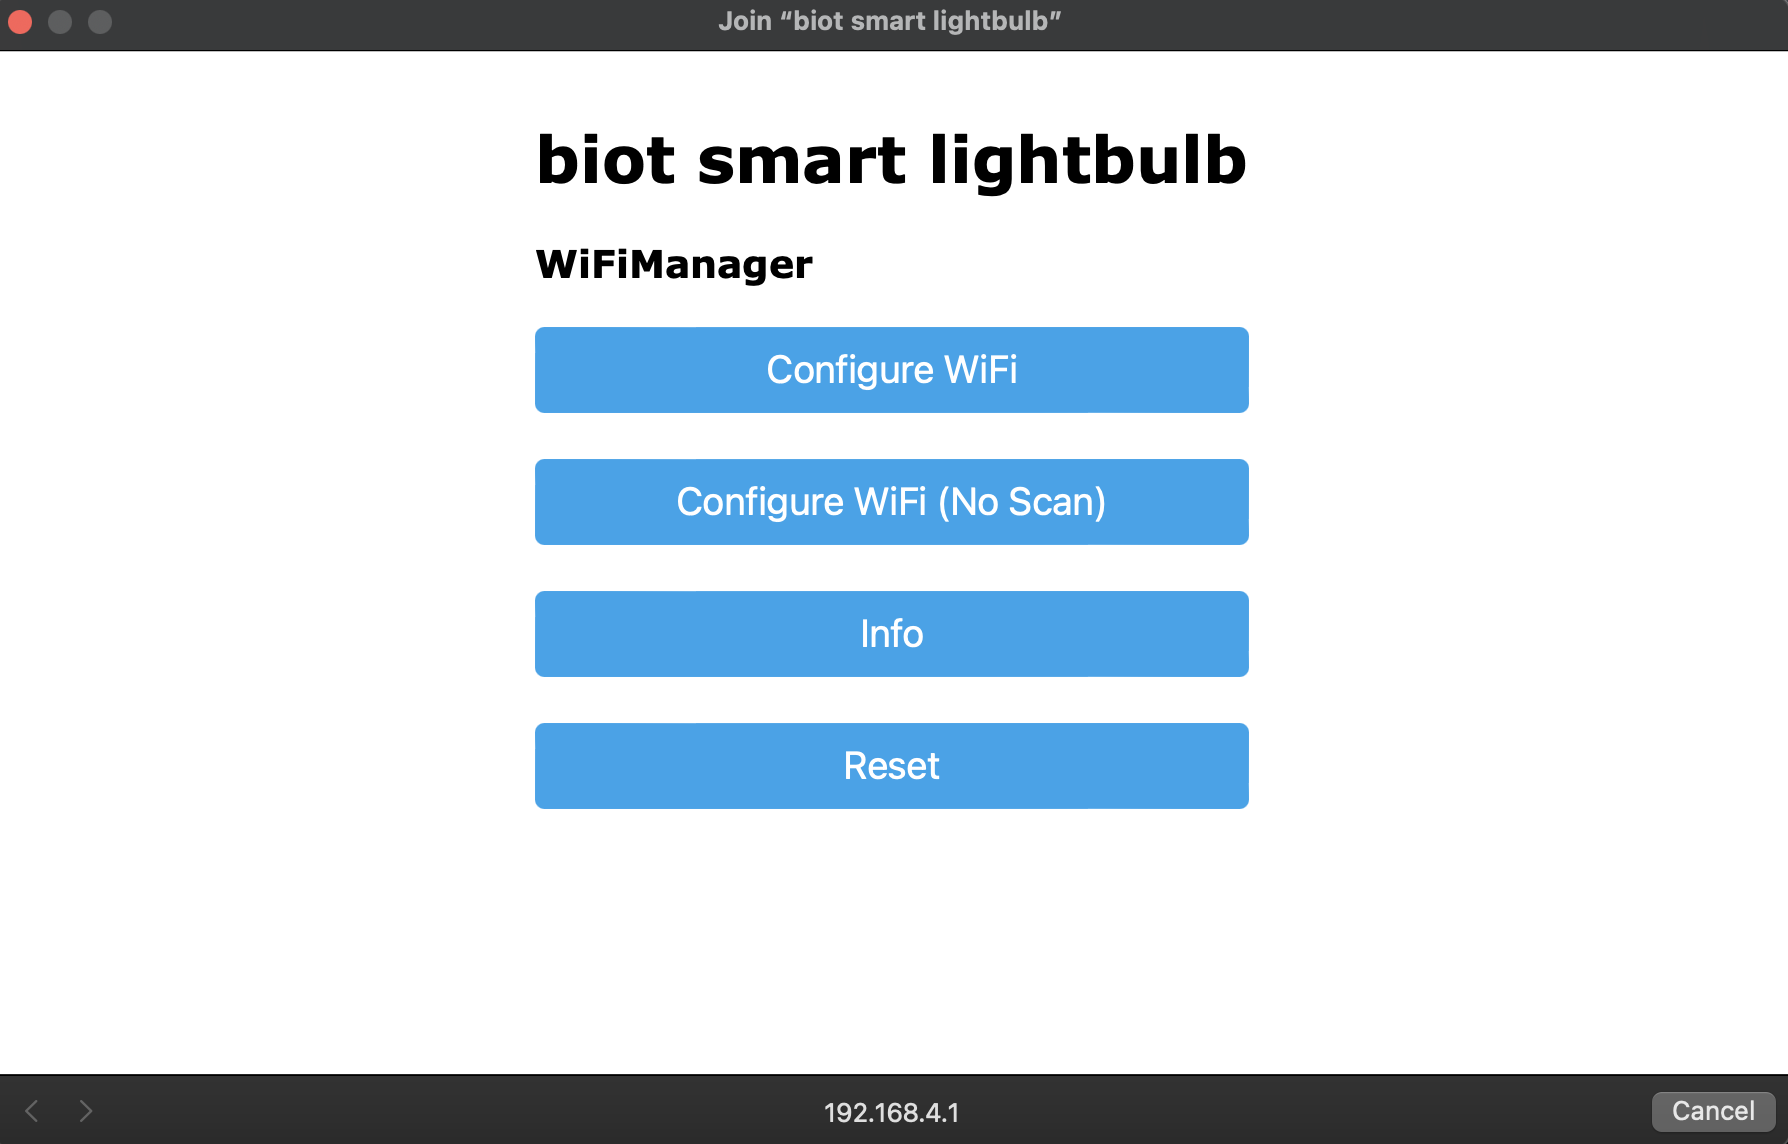
\includegraphics[scale=0.5]{resources/wifi-manager-1}
		\caption{Меню подключения умного устройства к Wi-Fi сети}
		\label{fig4.3}
	\end{figure}

	
	
	% добавить информацию о распределение ключа шифрования
	